\section{Direct Seed Filtering and Lower-Cost Model Inference}
\label{sec:native-acceleration}
The preceding comparisons show that a learned choice must save more
algebraic work than its prediction costs. We therefore changed the
interfaces between the frozen models and Kira, and measured the complete
reductions again. The seed interface can now select individual seeds
before Kira constructs their equations. We also tested a smaller set of
row choices that follows the form of the reduction model's training
examples. The original checkpoints remain unchanged.

\subsection{Relating the predicted seeds to Kira's targets}
A stored target can contain several integrals,
\begin{equation}
 \mathcal T_\nu=\sum_{\boldsymbol a\in\mathcal J_\nu}
 c_{\nu\boldsymbol a}(\boldsymbol x,d)I_{\boldsymbol a}.
 \label{eq:accel-expression}
\end{equation}
Here $\nu$ identifies a target, $\mathcal J_\nu$ is its set of component index vectors, and
$c_{\nu\boldsymbol a}$ is the known coefficient of each component.
The native interface asks Kira to reduce these components and then
combines their reductions with exact algebra. This procedure provides
two possible inputs for the seed model: the complete expression $\mathcal T_\nu$,
or each component $I_{\boldsymbol a}$ with coefficient one.

Let $\mathcal C$ be the stored candidate seed pool and let
$p_\theta(\boldsymbol b\mid \mathcal T_\nu)$ denote the frozen model's score for
seed $\boldsymbol b$, with the family and chosen masters also supplied.
For a threshold $\tau$, the expression-based seed set is
\begin{equation}
 \widehat{\mathcal S}_{\rm expr}(\tau)
 =\bigcup_\nu\{\boldsymbol b\in\mathcal C:
             p_\theta(\boldsymbol b\mid \mathcal T_\nu)\geq\tau\}.
\end{equation}
The component-based set instead uses
\begin{equation}
 \widehat{\mathcal S}_{\rm comp}(\tau)
 =\bigcup_{\boldsymbol a\in\cup_\nu\mathcal J_\nu}
 \{\boldsymbol b\in\mathcal C:
       p_\theta(\boldsymbol b\mid I_{\boldsymbol a})\geq\tau\}.
\end{equation}
Components already in the prescribed master basis need no prediction.
A seed set sufficient for the combined expression can differ from a set
sufficient for all components separately, since terms can cancel in
Eq.~\eqref{eq:accel-expression}. Both interfaces therefore require a
check of the final expression in the prescribed master basis.

We also test a local enlargement of a predicted set,
\begin{equation}
 \mathcal N_1(\mathcal S)
 =\left\{\boldsymbol b\in\mathcal C:
   \min_{\boldsymbol a\in\mathcal S}
   \sum_{i=1}^{N}|b_i-a_i|\leq1\right\}.
 \label{eq:seed-neighbours}
\end{equation}
Here $N$ is the number of family indices. This rule adds candidate seeds
that differ by one unit in one index. It supplies nearby IBP relations
without using the reference reduction. It gives no general proof that
the set suffices.

\subsection{Filtering before equation construction}
The earlier native adapter represented predictions by sector bounds.
Those bounds include intermediate seeds even when the model omitted
them. The new interface still supplies bounds that contain the chosen
seeds, but it also checks each seed vector before Kira constructs its
IBP equations. A vector outside the selected set contributes no IBP
equations through this call. Kira retains its symmetry handling,
equation selection, exact elimination and back substitution
\cite{Kira3}. The audit records both the allowed seed vectors and the
vectors that the generator actually used.

The model scores and the reference master coefficients serve separate
purposes. Predictions use only public family, target, master-label and
candidate information. After reduction, we check whether the target
contains any integral outside the prescribed master basis. An incomplete
learned attempt triggers a standard restricted native calculation within
the remaining time allowance. The final symbolic coefficients are then
compared with the recorded exact answer. Prediction, preparation,
unsuccessful attempts, fallback, target combination and exact checks
all contribute to the measured complete time.

\subsection{Reducing prediction costs and choosing a source row}
We exported the trained weights to a NumPy implementation of the same
layers. This removes the need to import the training framework for each
reduction, and it reuses the family, master and candidate embeddings
within a target batch. On 64 development targets, the seed probabilities
differed from the original implementation by at most
$4.18\times10^{-6}$, and every decision at threshold $0.5$ agreed.
Separate bounded feature checks verified the exported row network.
These checks concern numerical inference; exact reduction still comes
from Kira and the final coefficient checks.

For the row model, we first retained the full changing-matrix interface
of Section~\ref{sec:live-matrix} with the exported network. We then
restricted each decision to a source row for one current destination.
Using the leading-column group $R_{k_n}^{(n)}$ defined there, the largest
row identifier selects the destination $r_n$, and the model scores
\begin{equation}
 \mathcal A_n^{\rm source}
 =\{(q,r_n,k_n):q\in R_{k_n}^{(n)},\ q\ne r_n\}.
\end{equation}
The feature input contains the current rows in this group, with the
destination assigned the target role. Thus the model sees one changing
destination and its allowed sources, as in its training examples.
Kira applies the selected exact update from
Eq.~\eqref{eq:live-update}. The source can itself have changed in an
earlier step. The candidate count falls from $g(g-1)$ to $g-1$ for a
group of $g$ rows, while Kira's ordering still fixes the pivot column.
If the group contains only two rows, the supplied action set has one
element, so we apply that forced action without evaluating the network.

We also implemented the source-row network inside Kira's compiled
reduction code. Each choice reads the current rows directly, samples
their rational coefficients at the fixed finite-field point and forms
the same input features. The trained weights and features retain their
single-precision values, while the compiled layer arithmetic uses
double precision. An independent implementation with the same
arithmetic precision checks the probabilities, and development tests
also compare selected sources with the original single-precision
network. This numerical prediction only selects a valid source; Kira
continues to perform the rational row update exactly.

The compiled interface removes per-choice communication with a Python
process. It retains an audit of chosen rows and their probabilities,
and the measured time includes this audit. A combined method applies
both the learned seed filter and the compiled row policy during the
same reduction. An incomplete seed attempt uses the same exact
fallback rule as the seed-only method.


This restriction changes the model's supplied state and action set.
Its purpose is to reduce prediction work and test transfer to a
closer training configuration. It does not establish an optimal
elimination order, and its benefit must be measured against Kira's
native choices.

\subsection{Checking and expanding an incomplete seed set}
In separate development trials, we tested whether Kira's initial
finite-field master check could reject an incomplete seed set before
symbolic elimination \cite{Kira3}. This check compares the integrals
left by the generated system with the prescribed master basis. A
rejected set can then be enlarged before Kira starts the more expensive
symbolic calculation. The final coefficients still require exact
checks, since a numerical rank check alone does not prove the full
symbolic reduction. We retained the frozen policies in the reserved
comparison while testing these extensions.

For the first expansion rule, we rank each candidate seed by its
largest model score across the supplied expressions,
\begin{equation}
 Q_\theta(\boldsymbol b)
 =\max_\nu p_\theta(\boldsymbol b\mid\mathcal T_\nu).
\end{equation}
We begin with the first $k_0=32$ seeds and, after a rejected master
check, increase the budget according to
\begin{equation}
 k_{j+1}=\min(2k_j,|\mathcal C|).
\end{equation}
Here $j$ is the number of completed expansion steps and $\mathcal C$
is the candidate pool defined above. A control ranks seeds by their
smallest index distance to a component of a target expression, and
uses the same budget rule. The full candidate pool and restricted
native seeding provide two further controls.

A second rule begins with 64 seeds and uses the additional integrals
returned by the master check as new model inputs. Each such input
contains one integral with coefficient one. We add its four
highest-ranked unused candidates and repeat the check, using the full
pool after five rejected checks. A distance-based control applies the
same expansion to the same additional integrals. These checks require
every component to reduce in the prescribed basis, which can be
stricter than reducing the complete expression when terms cancel.

The 26 development trials gave 23 exact completions and three bounded
incomplete calculations. The latter used 64-target batches and affected
the native control and both learned variants in the initial check
experiment. All completed outputs passed 1104 independent
finite-field target checks. Across four complete 16-target comparisons,
the doubling rule with learned ranking took 1.022--1.422 times the
native control's complete time. In the subsequent residual-driven
trial, learned ranking reached a complete basis with 71 seeds,
while the distance control used 121. Its complete-time ratio
against native seeding was 0.996. These are single development
measurements; they do not establish a repeatable speedup for either
expansion strategy \cite{KiraNativeAccelerationData}.


\subsection{Development, validation and reserved comparisons}
We selected family instances before the new timing comparisons.
Development and adapter-validation instances use separate kinematic
groups from the original model-training partition. The reserved
cost-test instances come from the original test partition, and their
kinematic groups exclude every box group in the earlier cost comparison.
The network weights remain fixed throughout this selection.
The adapter-validation families belong to the original training
partition, so this stage selects an interface configuration and does
not measure generalization of the network itself. We performed
development comparisons on three of the reserved development
instances, selected the seed configuration on six validation instances
and then froze the policy before testing twelve instances from six
reserved kinematic groups.

All new native cases use symbolic reduction of one-loop box families
with independent propagator bases. Each case uses the same target expressions and master
basis for every method. Controls include restricted native seed bounds,
bounds taken directly from target indices, and the full stored candidate
pool with the individual-seed filter. These controls separate the
learned selection from changes to seed bounds or equation generation.

Every trial uses one computation thread with explicit time, memory and
scratch limits. We increased the array allowance from two simultaneous
jobs to four and then eight after checking the available node memory and project
storage. This changed the scheduling of independent trials while
preserving their individual resource limits and frozen policies. Methods run in rotated order on the same node for each
family and target-batch size. The retained-evidence limit interrupted some batches before a new trial could start; after lossless archive recompression, we resumed the missing trials on their original nodes and retained every completed observation. Every reserved method receives the same
initial 160-second native calculation allowance within a 180-second
complete-process limit. The memory and scratch limits are also the
same. We retain failed trials and report their completion status.
The validation rule assigns the 180-second total cap to an incomplete
trial when choosing the learned seed configuration. This capped score
is a selection rule; it is not a measured time for a completed
reduction. The reserved comparison uses the frozen configuration,
five repetitions and batches of 16 and 64 stored target expressions.
After an unsuccessful attempt, the remaining identical repetitions for
that method and batch are marked as skipped. Skipped repetitions receive
no measured time. Timing ratios require five successful repeats for both
methods, while completion and failure counts retain every attempted
case.

\subsection{Reserved results and exact checks}

\label{sec:acceleration-results}

The frozen comparison contains 720 planned records across twelve family instances, two target-batch sizes, six methods and five repetitions. We executed 616 trials and obtained 590 exact completions; the remaining 26 executed trials exceeded a resource limit or failed to complete. The early-stop rule left 104 repetitions unexecuted. These skipped records contain no timing measurement. The retained inputs, policy choices, successful reductions and failure records accompany the data release~\cite{KiraNativeAccelerationData}.

Validation selected the complete target expression with threshold $\tau=0.01$. This configuration and both trained checkpoints remained fixed during the reserved tests. Each method used the same master basis and targets in a batch.

For the three controls, restricted native Kira produced 105 exact completions, 3 failed trials and 12 skipped repetitions, the target-bound control produced 100 exact completions, 4 failed trials and 16 skipped repetitions, and the full candidate-pool control produced 105 exact completions, 3 failed trials and 12 skipped repetitions. These counts describe the bounded experiment and do not measure whether an unlimited calculation would complete.

Successful restricted-native trials took 10.54--112.46 seconds for the complete checked calculation. This range includes different family instances, target-batch sizes and CPU models. The paired ratios compare methods on the same node within each batch.

For the learned methods, the learned seed filter produced 100 exact completions, 4 failed trials and 16 skipped repetitions, the compiled row policy produced 105 exact completions, 3 failed trials and 12 skipped repetitions, and the combined method produced 75 exact completions, 9 failed trials and 36 skipped repetitions. Completed seed and combined trials used the standard fallback 30 and 50 times, respectively.

Every completed final expression matched its recorded rational master coefficients. The independent audit performed 67,920 additional master-coefficient sample checks and 65,355 exact-row sample checks. It checked 11,405 compiled model choices and 10,380 forced source actions. Trace checks cover completed native attempts; 55 failed attempts had incomplete traces. The final coefficient checks still apply to any successful fallback. Input and checkpoint hashes agree with the values frozen before testing.

\subsection{Complete reduction time and algebraic work}

For each family and batch size, we take the median of five successful repetitions. We then form the ratio of learned time to control time and report the geometric mean across complete paired batches. A ratio below one means a lower measured time. We resample complete kinematic groups 10,000 times to obtain descriptive 95\% intervals, keeping related profiles and batch sizes together. These intervals describe the completed subset of this small collection; failed and skipped trials remain in the completion counts above.

Restricted native Kira completed all five repetitions in 1 batches where the learned seed filter did not, while the learned seed filter completed all five repetitions in 0 batches where that control did not.

The learned seed filter has a complete-time ratio of 1.295 (descriptive 95\% interval 1.156--1.542; 20 batches) against restricted native Kira. Its native-calculation subtotal, including seed prediction when used, has ratio 1.400 (descriptive 95\% interval 1.201--1.816; 20 batches). The subtotal excludes input preparation, final target combination and verification, which remain included in the complete time.

Restricted native Kira completed all five repetitions in 0 batches where the compiled row policy did not, while the compiled row policy completed all five repetitions in 0 batches where that control did not.

The compiled row policy has a complete-time ratio of 1.024 (descriptive 95\% interval 0.998--1.053; 21 batches) against restricted native Kira. Its native-calculation subtotal, including seed prediction when used, has ratio 1.025 (descriptive 95\% interval 1.001--1.078; 17 batches). The subtotal excludes input preparation, final target combination and verification, which remain included in the complete time.

Restricted native Kira completed all five repetitions in 6 batches where the combined method did not, while the combined method completed all five repetitions in 0 batches where that control did not.

The combined method has a complete-time ratio of 1.983 (descriptive 95\% interval 1.575--2.476; 15 batches) against restricted native Kira. Its native-calculation subtotal, including seed prediction when used, has ratio 2.289 (descriptive 95\% interval 1.247--3.673; 8 batches). The subtotal excludes input preparation, final target combination and verification, which remain included in the complete time.

Against the target-bound control, complete-time ratios are 0.902 (descriptive 95\% interval 0.711--1.163; 20 batches), 0.712 (descriptive 95\% interval 0.597--0.864; 20 batches), 1.415 (descriptive 95\% interval 0.902--2.160; 14 batches), in seed, row and combined order. Against the full candidate-pool control, the corresponding ratios are 1.317 (descriptive 95\% interval 1.167--1.569; 20 batches), 1.040 (descriptive 95\% interval 1.016--1.061; 21 batches), 2.028 (descriptive 95\% interval 1.565--2.616; 15 batches). Each ratio uses its own complete paired cohort, so comparisons with different failure patterns can contain different batches.

\begin{figure}[htbp]
\centering
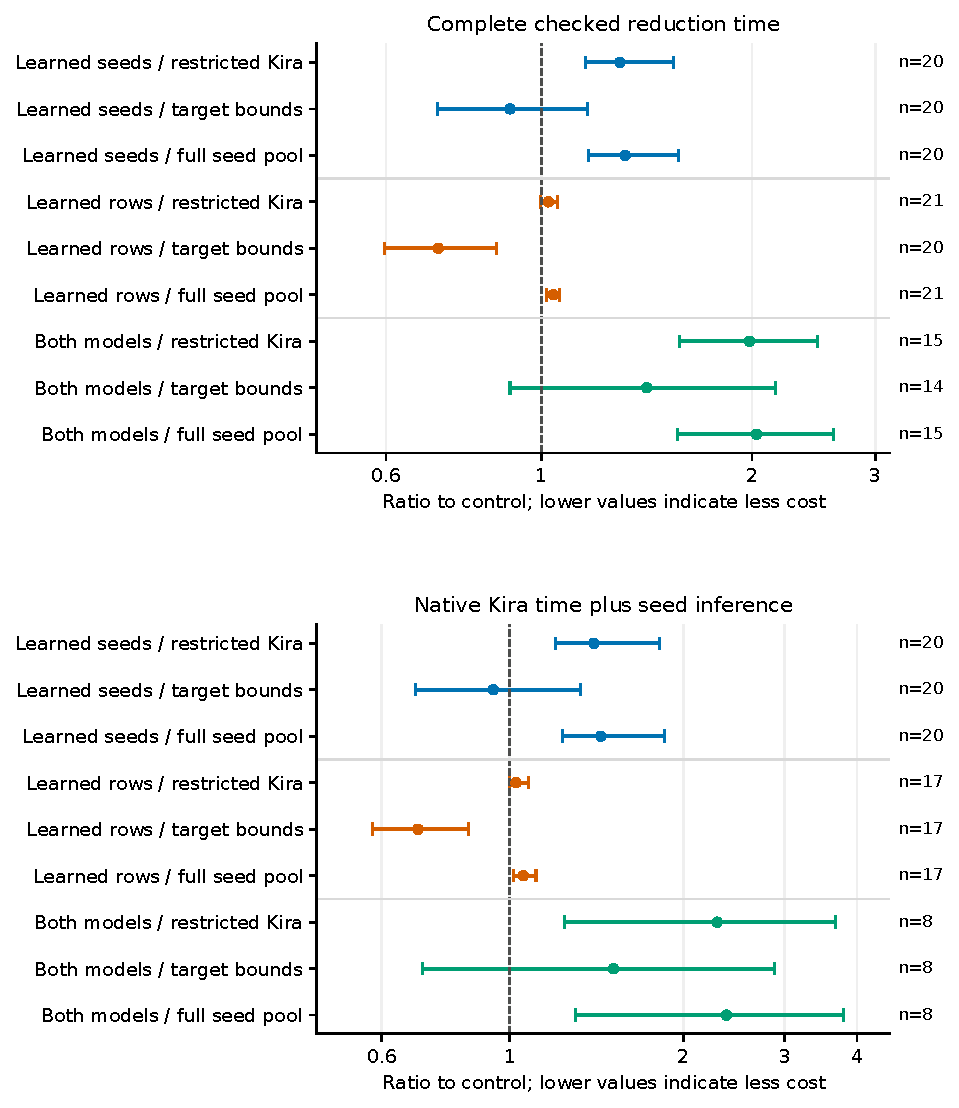
\includegraphics[width=\linewidth]{figures/native_acceleration_times.pdf}
\caption{Learned-to-control time ratios in the reserved native comparison.
The upper panel includes the complete checked reduction, and the lower panel
shows the native subprocess subtotal plus seed prediction. Points show
geometric mean ratios and lines show descriptive intervals obtained by
resampling kinematic groups. The label $n$ gives the number of paired
batches with five successful repeats for both methods.}
\label{fig:native-acceleration-time}
\end{figure}

The learned seed filter has a generated-equation ratio of 0.168 (descriptive 95\% interval 0.097--0.294; 20 batches), a selected-equation ratio of 0.982 (descriptive 95\% interval 0.797--1.205; 20 batches) and a forward-update ratio of 3.575 (descriptive 95\% interval 2.647--5.211; 20 batches) against restricted native Kira. These are counters from the native reduction passes, including completed fallback passes.

The compiled row policy has a generated-equation ratio of 1.141 (descriptive 95\% interval 1.032--1.275; 21 batches), a selected-equation ratio of 1.141 (descriptive 95\% interval 1.032--1.275; 21 batches) and a forward-update ratio of 0.905 (descriptive 95\% interval 0.840--0.972; 17 batches) against restricted native Kira. These are counters from the native reduction passes, including completed fallback passes.

The combined method has a generated-equation ratio of 0.462 (descriptive 95\% interval 0.254--0.745; 15 batches), a selected-equation ratio of 1.341 (descriptive 95\% interval 1.080--1.582; 15 batches) and a forward-update ratio of 2.363 (descriptive 95\% interval 1.041--4.534; 8 batches) against restricted native Kira. These are counters from the native reduction passes, including completed fallback passes.

Generation counters count equations reported in successive generation passes and can include repeated equations. A forward update is one committed elimination step; this count does not measure every polynomial or rational-function operation. Failed attempts can have truncated work counters, so the complete time and completion status remain the primary measures.

\begin{figure}[htbp]
\centering
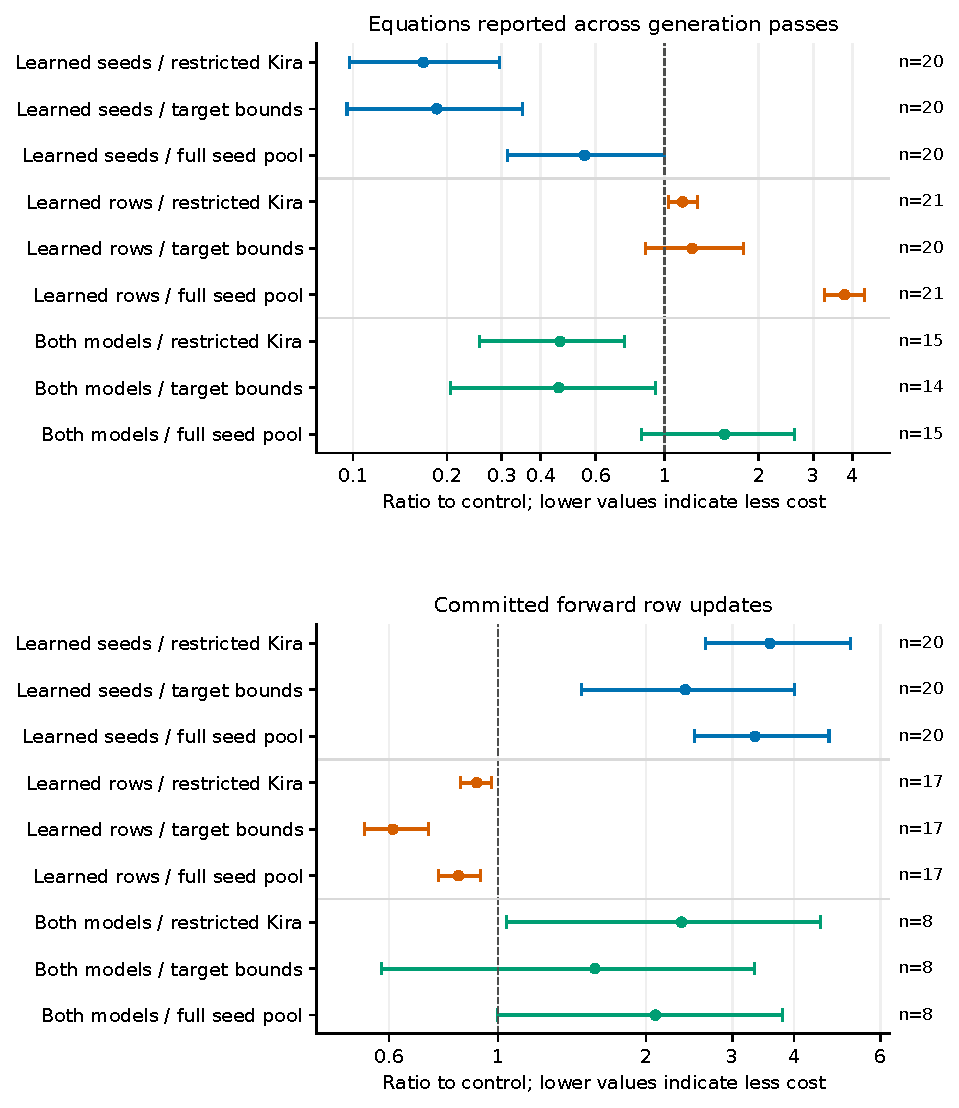
\includegraphics[width=\linewidth]{figures/native_acceleration_work.pdf}
\caption{Generated-equation and forward-update ratios on complete paired
batches. The controls and cohort labels follow
Fig.~\ref{fig:native-acceleration-time}. These counters measure reported
generation work and committed updates, while symbolic coefficient
complexity can change the cost of each update.}
\label{fig:native-acceleration-work}
\end{figure}
\FloatBarrier

\subsection{Numerical inference and scope of the result}

The compiled-model development audit checked 256 action feature vectors and 2,247 sampled coefficients. The maximum feature difference was 0, and the largest probability difference from the independent double-precision calculation was $1.41\times10^{-13}$. All selected sources agreed with the original single-precision model in these development trials. The separate maximum probability difference from that original arithmetic was $1.6\times10^{-05}$.

The largest sampled process-tree memory was 0.506 GB, and the largest trial scratch directory was 49.29 MB. The bounded runs kept their scientific records and model files on Hoffman; the report contains the derived plots and results.

The complete paired comparisons do not show a lower aggregate runtime than restricted native Kira for these learned methods. Lower inference costs alone do not ensure that the chosen seeds and rows save enough algebraic work. The new native tests cover one-loop boxes and do not establish performance on independent high-loop scattering families. The existing weights were trained to recover recorded seed sets and row choices, and Section~\ref{sec:complete-multiloop} reports a separate cost-trained policy on native Kira trajectories.

\subsection{Transfer to a two-loop propagator family}
We also applied the unchanged interfaces to the massless two-loop
propagator family used in the earlier cost comparisons. Its five
independent family indices fit the compiled row interface. We fixed
two batches of 16 and 64 stored target expressions and all policies
before this transfer calculation. Each method uses five rotated
repetitions, the same master basis and the same time and memory limits.
Storage-interrupted trials resume on their original node, with earlier
observations preserved. Because this family appeared in earlier
comparisons, this experiment measures transfer of the revised
implementation and does not establish generalization to a newly unseen
family.

Alongside native seeding and the full candidate pool, we include a
deterministic source-row control using the same compiled reduction
structure. This control selects a source by row length and integral ordering
within the same changing leading-column group. Comparing the learned row policy
with this control separates the source choice from changes to the
compiled reduction structure. Every completed reduction receives the
same exact coefficient check and an independent finite-field check.

The transfer experiment contains 60 measured trials among 60 planned records, with 60 exact completions. The independent audit performed 7,200 target-coefficient checks and 2,355 row-update checks.

For 16 targets, the native control's median complete time was $12.003$ seconds. The learned seed filter gave a time ratio of $0.992$ with descriptive interval $[0.962,1.030]$; the learned source-row policy gave a time ratio of $0.991$ with descriptive interval $[0.984,1.022]$; the combined policy gave a time ratio of $0.976$ with descriptive interval $[0.961,0.996]$. In the matched controls, the learned seed filter relative to the full pool had ratio $1.051$ with interval $[1.024,1.072]$ and the learned source choice relative to the deterministic compiled control had ratio $0.987$ with interval $[0.979,1.034]$.

For 64 targets, the native control's median complete time was $12.770$ seconds. The learned seed filter gave a time ratio of $1.758$ with descriptive interval $[1.744,1.777]$; the learned source-row policy gave a time ratio of $0.976$ with descriptive interval $[0.964,0.992]$; the combined policy gave a time ratio of $1.755$ with descriptive interval $[1.740,1.777]$. In the matched controls, the learned seed filter relative to the full pool had ratio $1.907$ with interval $[1.880,1.920]$ and the learned source choice relative to the deterministic compiled control had ratio $0.987$ with interval $[0.952,1.012]$.


The compiled learned-row pipeline reduced the median complete time for
64 targets from 12.770 to 12.460 seconds, a measured reduction of
2.4\%. Its ratio against the deterministic compiled control has an
interval that includes one, so this experiment does not resolve a
benefit caused by the learned source choice itself. The full-pool
control was faster, at 11.773 seconds. For 16 targets, the combined
pipeline reduced the native median by 2.4\%, but the full-pool control
again completed sooner. For 64 targets, every learned-seed and combined
trial required fallback, whose cost is included in the reported time.
These observations establish limited gains relative to the stated
native baseline and also identify stronger deterministic controls.


Figure~\ref{fig:native-transfer} shows all complete paired comparisons.
A ratio below one denotes a lower median complete time. The intervals
come from 10,000 paired resamples of the five repetitions and describe
repeat-to-repeat variation within this one family. They do not measure
uncertainty across different integral families. Incomplete pairs remain
in the completion counts and receive no timing ratio
\cite{KiraNativeAccelerationData}.

\begin{figure}[htbp]
 \centering
 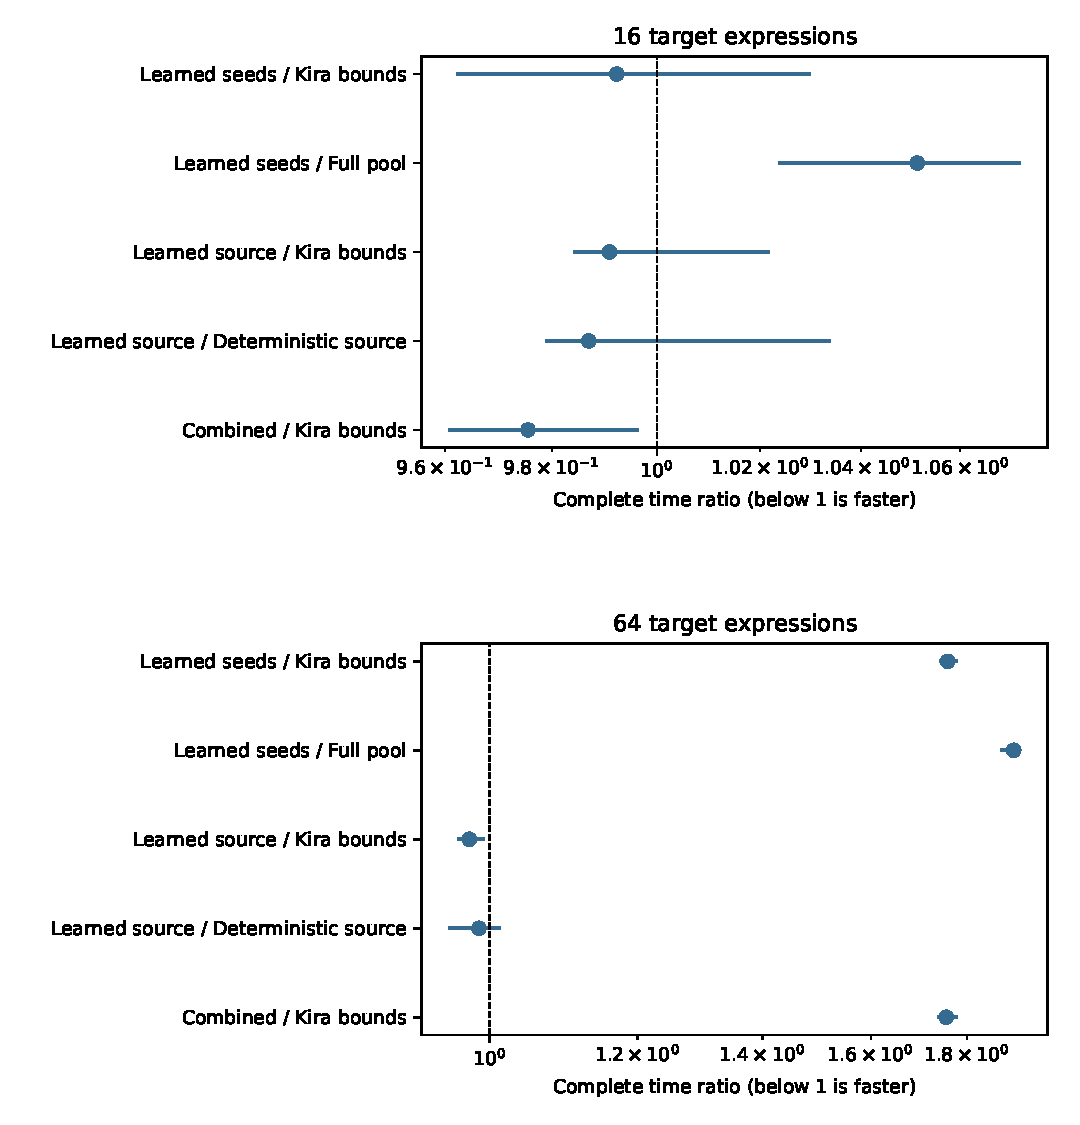
\includegraphics[width=\textwidth]{figures/native_transfer_times.pdf}
 \caption{Complete-time ratios in the two-loop transfer comparison for
 16 targets (upper panel) and 64 targets (lower panel). Points show
 ratios of five-repeat medians, and bars show descriptive paired-repeat
 intervals. All times include prediction, target preparation, exact
 reduction, combination, checks and any required fallback.}
 \label{fig:native-transfer}
\end{figure}


\subsection{Applying the seed model to complete target expressions}
The native interface reduces each component of
Eq.~\eqref{eq:accel-expression} before combining the result. We also
applied the fast seed model directly to that complete expression,
using Kira's supplied-equation mode. This tests the form of the target
used to train the seed model and allows cancellations between its
components during the reduction.

Let $\mathcal E_{\boldsymbol b}$ be the stored IBP identities generated
from candidate seed $\boldsymbol b$, and let
$\mathcal E_{\rm bg}$ contain the stored symmetry and other background
identities. The selected equation set is
\begin{equation}
 \mathcal E(\mathcal S)=\mathcal E_{\rm bg}\cup
       \bigcup_{\boldsymbol b\in\mathcal S}\mathcal E_{\boldsymbol b}.
\end{equation}
For each requested expression, we add its defining relation
\begin{equation}
 \mathcal T_\nu-
 \sum_{\boldsymbol a\in\mathcal J_\nu}
 c_{\nu\boldsymbol a}I_{\boldsymbol a}=0.
\end{equation}
Kira eliminates the supplied system with the target expressions ordered
above their component integrals and the prescribed masters preferred
at the end of the ordering. It therefore obtains the master expansion
of $\mathcal T_\nu$ in one exact solve. The same public identity pool,
target definitions and master basis enter every compared method.

The model takes the union of candidates whose score reaches
$\tau=0.01$, using the unchanged weights and the fast inference
implementation. We tested this set both with and without an early
finite-field master check. An incomplete selected system triggers a
full-pool calculation within the remaining time allowance. The early
check compares the remaining integrals with the prescribed master
basis; exact final coefficient checks still determine whether the requested reductions
agree with their recorded answers. A global master check can require
more relations than a particular target combination needs.

These calculations begin with stored IBP identities, whose prior
generation cost is excluded for every method. The measured complete
time includes loading those inputs, prediction, equation selection and
export, Kira's exact calculation, admission checks when used, failed
attempts, fallback and final verification. Thus the result concerns
repeated reduction from a common identity pool. It does not measure
native generation of a new family's equations.


The separate development and adapter-validation collection contains 80 trials, with 74 exact completions and 6 incomplete calculations. Independent checks evaluated 2,013 target coefficients at stored finite-field points. The six adapter-validation family instances belong to the original training partition and use two batch sizes, one and sixteen targets. We retained every measured cost and selected a learned interface only when its geometric mean complete-time ratio to the full-pool control was below one and it preserved every control completion.

The validation ratio without the early master check was 1.113 across 11 complete paired batches. The full-pool control completed 0 additional batches that this learned interface did not complete. These single validation measurements select the interface and do not establish a repeatable timing gain.

The validation ratio with the early master check was 0.930 across 11 complete paired batches. The full-pool control completed 0 additional batches that this learned interface did not complete. These single validation measurements select the interface and do not establish a repeatable timing gain.

\subsection{Reserved tests of complete-expression reduction}

Validation selected the early master check. We froze this choice before applying it to the twelve original-held-out box instances used in the native comparison. The network weights and threshold remain fixed. Each instance supplies batches of one and sixteen target expressions, with five rotated repetitions per method on the same node. These are reused physical families and constructed targets; the new comparison tests the revised interface on original-held-out model data.

The controls use the full stored identity pool and a fixed set of 64 seeds ranked by their smallest index distance to any target component. The distance control uses the same exact reduction and full-pool fallback as the learned method. This first distance control proceeds directly to symbolic elimination, while the selected learned method uses the early master check. Their time ratio therefore includes both seed selection and the difference in admission checks.

The frozen plan contains 360 records. We executed 348 trials and obtained 345 exact completions; 3 measured trials failed to complete within the bounds, and 12 remaining repeats were skipped after an earlier failure. Every completed master expansion matched its exact reference, and the independent audit checked 8,460 target coefficients directly against the exported Kira reductions. Skipped repetitions have no assigned runtime.

The learned interface produced 115 exact completions, 1 failed trial and 4 skipped repeats. Completed trials used fallback 25 times.

The full-pool control produced 115 exact completions, 1 failed trial and 4 skipped repeats. Completed trials used fallback 0 times.

The distance control produced 115 exact completions, 1 failed trial and 4 skipped repeats. Completed trials used fallback 55 times.

We form a median from five successful repetitions for each method and batch, and take geometric mean ratios over complete paired batches. Descriptive 95\% intervals resample the six kinematic groups 10,000 times, preserving the relationship between profiles and batch sizes. Completion losses remain separate from these ratios.

The learned interface has a complete-time ratio of 0.944 against the full-pool control, with descriptive interval $[0.863,1.042]$ across 23 paired batches. The control completed all repeats in 0 additional batches, and the learned method completed all repeats in 0 additional batches.

The learned interface has a complete-time ratio of 0.604 against the distance control, with descriptive interval $[0.534,0.678]$ across 23 paired batches. The control completed all repeats in 0 additional batches, and the learned method completed all repeats in 0 additional batches.

The observed geometric mean complete time is 5.6\% lower than the full-pool Kira control on batches where both methods completed all five repetitions. Because the descriptive interval includes one, the aggregate timing gain across both batch sizes remains uncertain. The result applies to these constructed target expressions and their existing identity pools; it does not establish a speedup for general multiloop amplitude reductions \cite{KiraNativeAccelerationData}.

\begin{figure}[htbp]
\centering
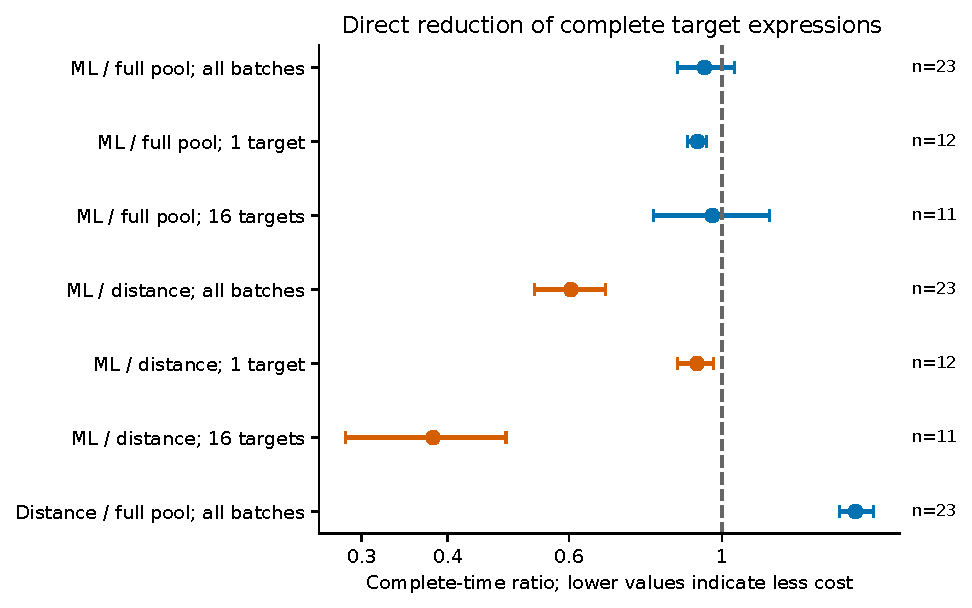
\includegraphics[width=\linewidth]{figures/whole_expression_times.pdf}
\caption{Complete-time ratios for direct reduction of complete target
expressions. Points show geometric means of five-repeat median ratios,
and intervals resample kinematic groups. The label $n$ gives the
number of complete paired batches. Failed and skipped trials remain
in the completion counts.}
\label{fig:whole-expression-time}
\end{figure}
\FloatBarrier



\subsection{Using the same master check for both seed selectors}
The preceding distance control enters symbolic elimination directly,
while the learned method first checks the selected master basis.
To compare seed choices under the same admission procedure, we fixed
a second confirmation in which both selected sets receive the same
early check and full-pool fallback. The learned scores, threshold,
distance rule, twelve family instances and target batches stay
unchanged. The full-pool Kira control again uses its standard
supplied-equation reduction. We retained every measurement in the
first comparison.

Each method again uses five rotated repetitions on the same node
within a family and batch. This new comparison contains independent
timing repetitions of the same physical cases, so it checks the effect
of matching the admission procedure and does not introduce new
integral families. Complete times and descriptive intervals follow
the definitions in the preceding subsection.


The comparison with the same early check contains 360 records, of which 348 are measured trials. It produced 345 exact completions, 3 incomplete measured trials and 12 skipped repetitions. Independent checks evaluated 8,460 target coefficients against the raw Kira exports. All completed reductions matched their exact reference coefficients.

The learned method completed 115 trials exactly, with 1 failed trial and 4 skipped repetitions. Its completed trials required fallback 25 times.

The full-pool control completed 115 trials exactly, with 1 failed trial and 4 skipped repetitions. Its completed trials required fallback 0 times.

The distance control with the early check completed 115 trials exactly, with 1 failed trial and 4 skipped repetitions. Its completed trials required fallback 55 times.

Across both batch sizes, the learned complete-time ratio to the full-pool control is 0.932, with descriptive interval $[0.845,1.031]$ across 23 paired batches. The control completed 0 additional batches, while the learned method completed 0 additional batches.

For batches of 1 target, the learned complete-time ratio to the full-pool control is 0.914, with descriptive interval $[0.871,0.958]$ across 12 paired batches. The control completed 0 additional batches, while the learned method completed 0 additional batches.

For batches of 16 targets, the learned complete-time ratio to the full-pool control is 0.952, with descriptive interval $[0.772,1.148]$ across 11 paired batches. The control completed 0 additional batches, while the learned method completed 0 additional batches.

Across both batch sizes, the learned complete-time ratio to the distance control with the same early check is 0.925, with descriptive interval $[0.848,1.024]$ across 23 paired batches. The control completed 0 additional batches, while the learned method completed 0 additional batches.

For batches of 1 target, the learned complete-time ratio to the distance control with the same early check is 0.913, with descriptive interval $[0.855,0.972]$ across 12 paired batches. The control completed 0 additional batches, while the learned method completed 0 additional batches.

For batches of 16 targets, the learned complete-time ratio to the distance control with the same early check is 0.939, with descriptive interval $[0.764,1.136]$ across 11 paired batches. The control completed 0 additional batches, while the learned method completed 0 additional batches.

For the predefined single-target comparison, the learned method reduced geometric mean complete time by 8.6\% relative to the full pool and by 8.7\% relative to the distance rule with the same early check. Both descriptive intervals lie below one, and every method completed all five repeats for all twelve instances. The first confirmation gave a 7.8\% reduction relative to the full pool for this batch size. These results support a repeated gain for one constructed target expression at a time in this stored-identity setting. The sixteen-target intervals include one, so that batch size does not establish a consistent gain. The geometric means of the twelve per-family median complete times were 5.478 seconds for the full pool and 5.005 seconds for the learned method.

The learned workflow has an observed 6.8\% lower geometric mean complete time than the full-pool Kira control on batches where both methods completed all five repetitions. Because the descriptive interval includes one, the aggregate timing gain across both batch sizes remains uncertain. These conclusions concern reduction from the supplied identity pools and the tested constructed target expressions. Native equation generation, arbitrary scattering amplitudes and larger independent multiloop families remain outside this result \cite{KiraNativeAccelerationData}.

\begin{figure}[htbp]
\centering
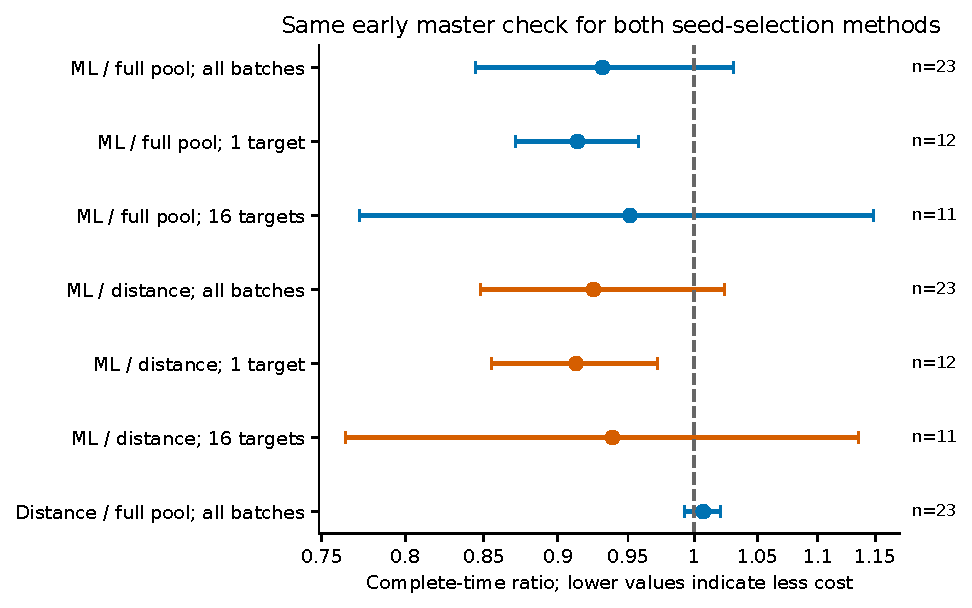
\includegraphics[width=\linewidth]{figures/whole_expression_matched_times.pdf}
\caption{Complete-time ratios with the same early master check for
learned and distance-selected seeds. Points show geometric means
of five-repeat median ratios, intervals resample kinematic groups,
and $n$ gives the number of complete paired batches. The full-pool
control uses standard supplied-equation Kira reduction.}
\label{fig:whole-expression-matched}
\end{figure}
\FloatBarrier


